[introduction/in-intro.tex]
\section{DAQ for CBM}

The communication and processing needed between the front-end electronics,
generating digitized detector information, and the archival storage, where
the complete context of selected candidate events is recorded, can be
structured and organized in several ways.
The solution described in \cite{CBM-stat-rep} is guided by two principles:
processing is done after event building and it is done in a
structured processor farm.
It is well adapted to the type of processing needed in the CBM experiment
and leads to a straightforward and modular architecture.

\begin{figure}[htb]
\centering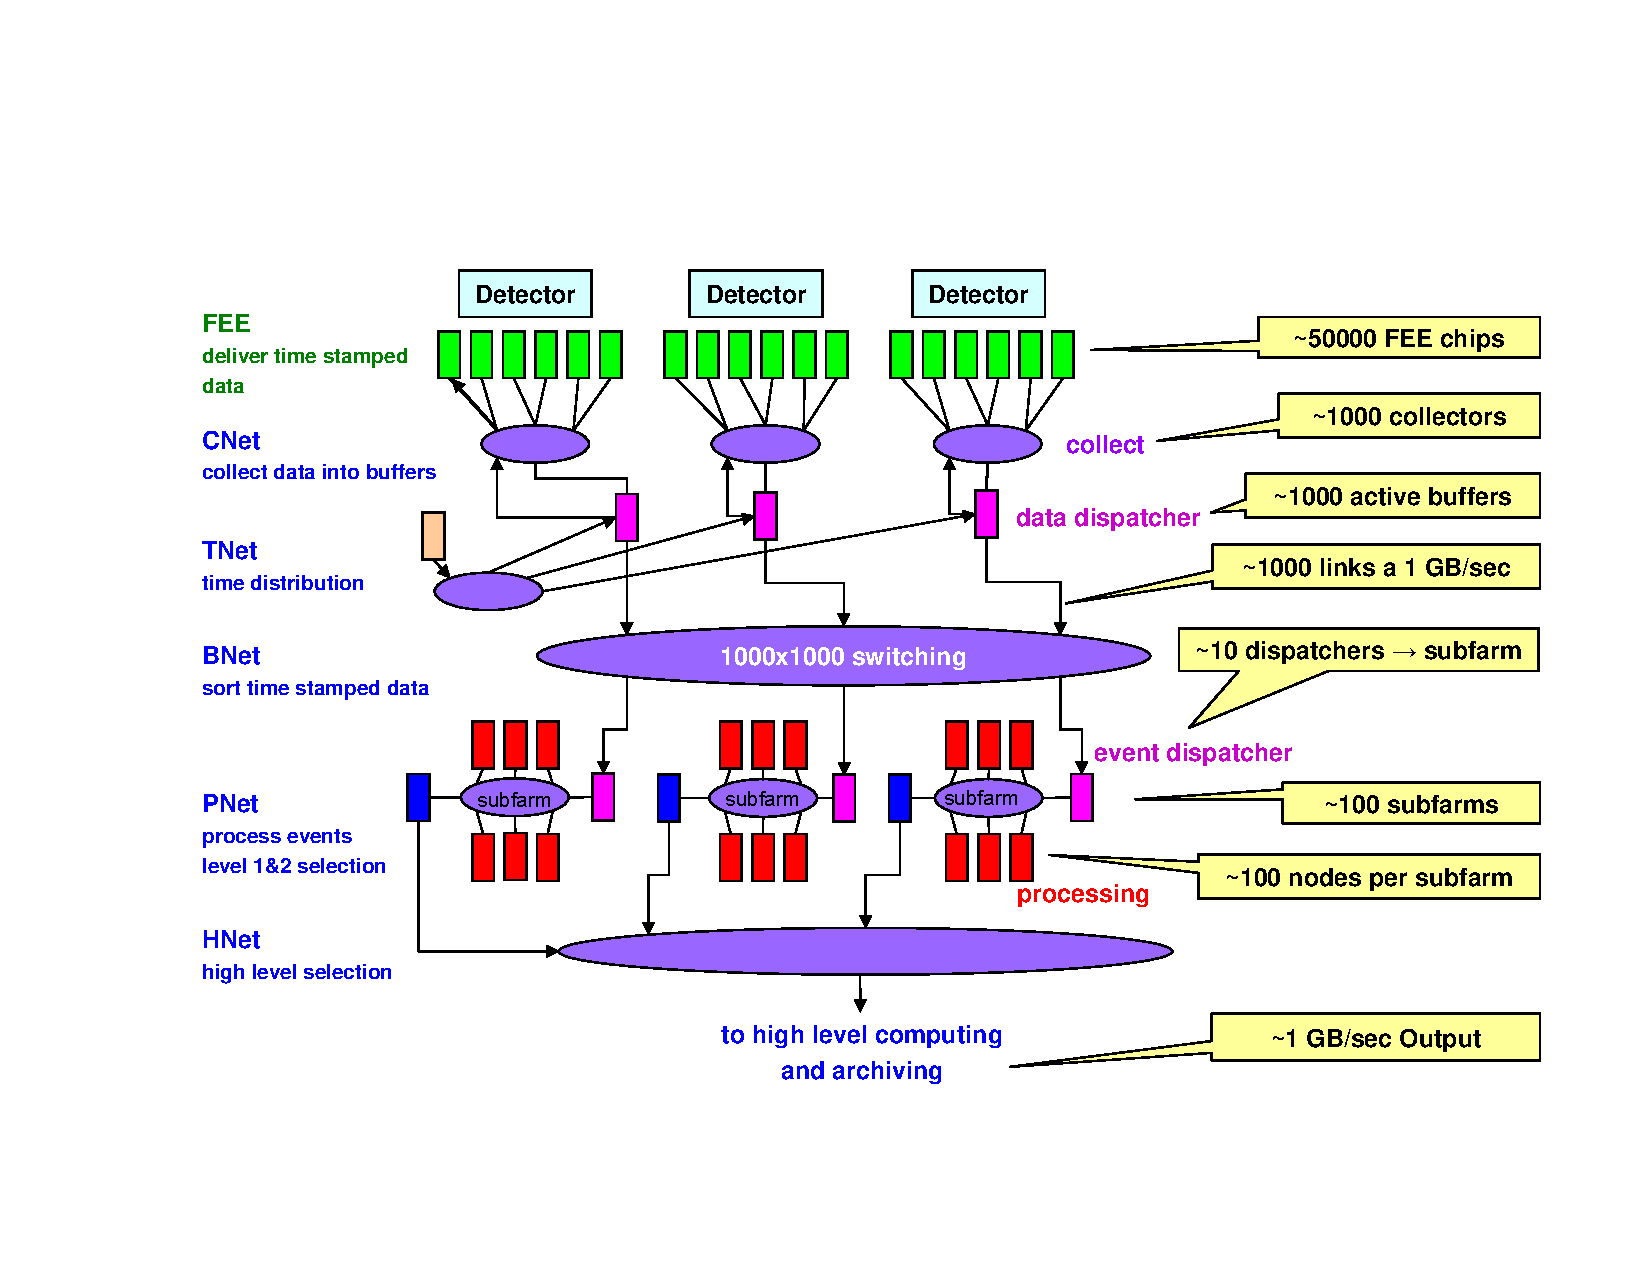
\includegraphics[width=.8\textwidth]
{dabcf-daq-all}
\caption{CBM overall data processing architecture}
\label{fig:daq-all}
\end{figure}

A logical data flow diagram is shown in Fig.~\ref{fig:daq-all},
indicating the data sources and processing elements as boxes and every
form of interconnection networks as ovals.
\clearpage

\section{Demonstrator mission}
\index{Demonstrator!mission}
\hyperdef{in}{mission}{[Marker:in.mission]}\\
The final DAQ system will be quite complex and involves many
technologies which are at the limits of today possibilities.
Therefore it is necessary to start early with a system which can
be implemented in the next years without showing up the full final
performance needed. This system, a \DDA, is useful in four
respects.
\subsection{Demonstration of key technologies}
\index{Demonstrator!technology}
The first task is to prove the key technologies needed, maybe with
less performance.
\begin{compactitem}[$\bullet$]
\item FEE: self-triggered, data push, conditional RoI based readout
\item CNet: combined data, time, control, and RoI traffic
\item TNet: low jitter clock and synchronization over serial links
\item BNet: high bandwidth switched network for event building
\item ECS: integrated control system
\end{compactitem}
\subsection{Test bed for prototypes}
All components will need iterations. A testing environment is
needed from the beginning.
\begin{compactitem}[$\bullet$]
\item Hardware
\item Firmware
\item Controls
\item Software
\end{compactitem}
\subsection{Functional DAQ for detector tests}
There are many questions concerning detector performance.
Prototypes will be developed. They can only be tested with a DAQ
system with the same characteristics as the final one. The whole
readout chain must be available to prove that a triggerless
readout is feasible.
\subsection{General purpose DAQ for medium sized experiments}
To prove that a highly distributed system scales it is necessary
to install at least a medium sized setup. This can only be
afforded if it is used in production for an experiment.

\section{Demonstrator use cases}
\index{Demonstrator!use cases}
According the mission there are several use cases or scenarios:
\subsubsection{Frontend test bed}
The new components FEB, DCB, and ABB and their connections must be tested.
The timing system and the triggered/non-triggered mode must be tested.
\subsubsection{Detector test bed}
Detector tests with a free running system are needed to verify that the data rates
are not very much bigger that expected (dark noise).
\subsubsection{Switched event building}
Independent of the data sources (ABB or GEB) several mechanisms for the switched
event building must be implemented and tested.
\subsubsection{DAQ framework and control systems}
There are still several options for the choice of the control system.
\subsubsection{MBS replacement}
\index{Demonstrator!MBS}
Very probably there will be no complete replacement of the \mbs~ possible for the next years.
One could envision that the \mbs~ frontend nodes, i.e. the readout nodes
send their subevent data peer to peer to new event builder nodes (new \mbs~ mode).
\subsubsection{Hybrid setup}
If the system should run in production, very probably a hybrid of \mbs~ for ancillary components
and new frontends will be needed.

\section{Demonstrator architecture}
As a first step the \DDA~ shall be used to investigate practically the technologies needed.

\begin{figure}[htb]
\centering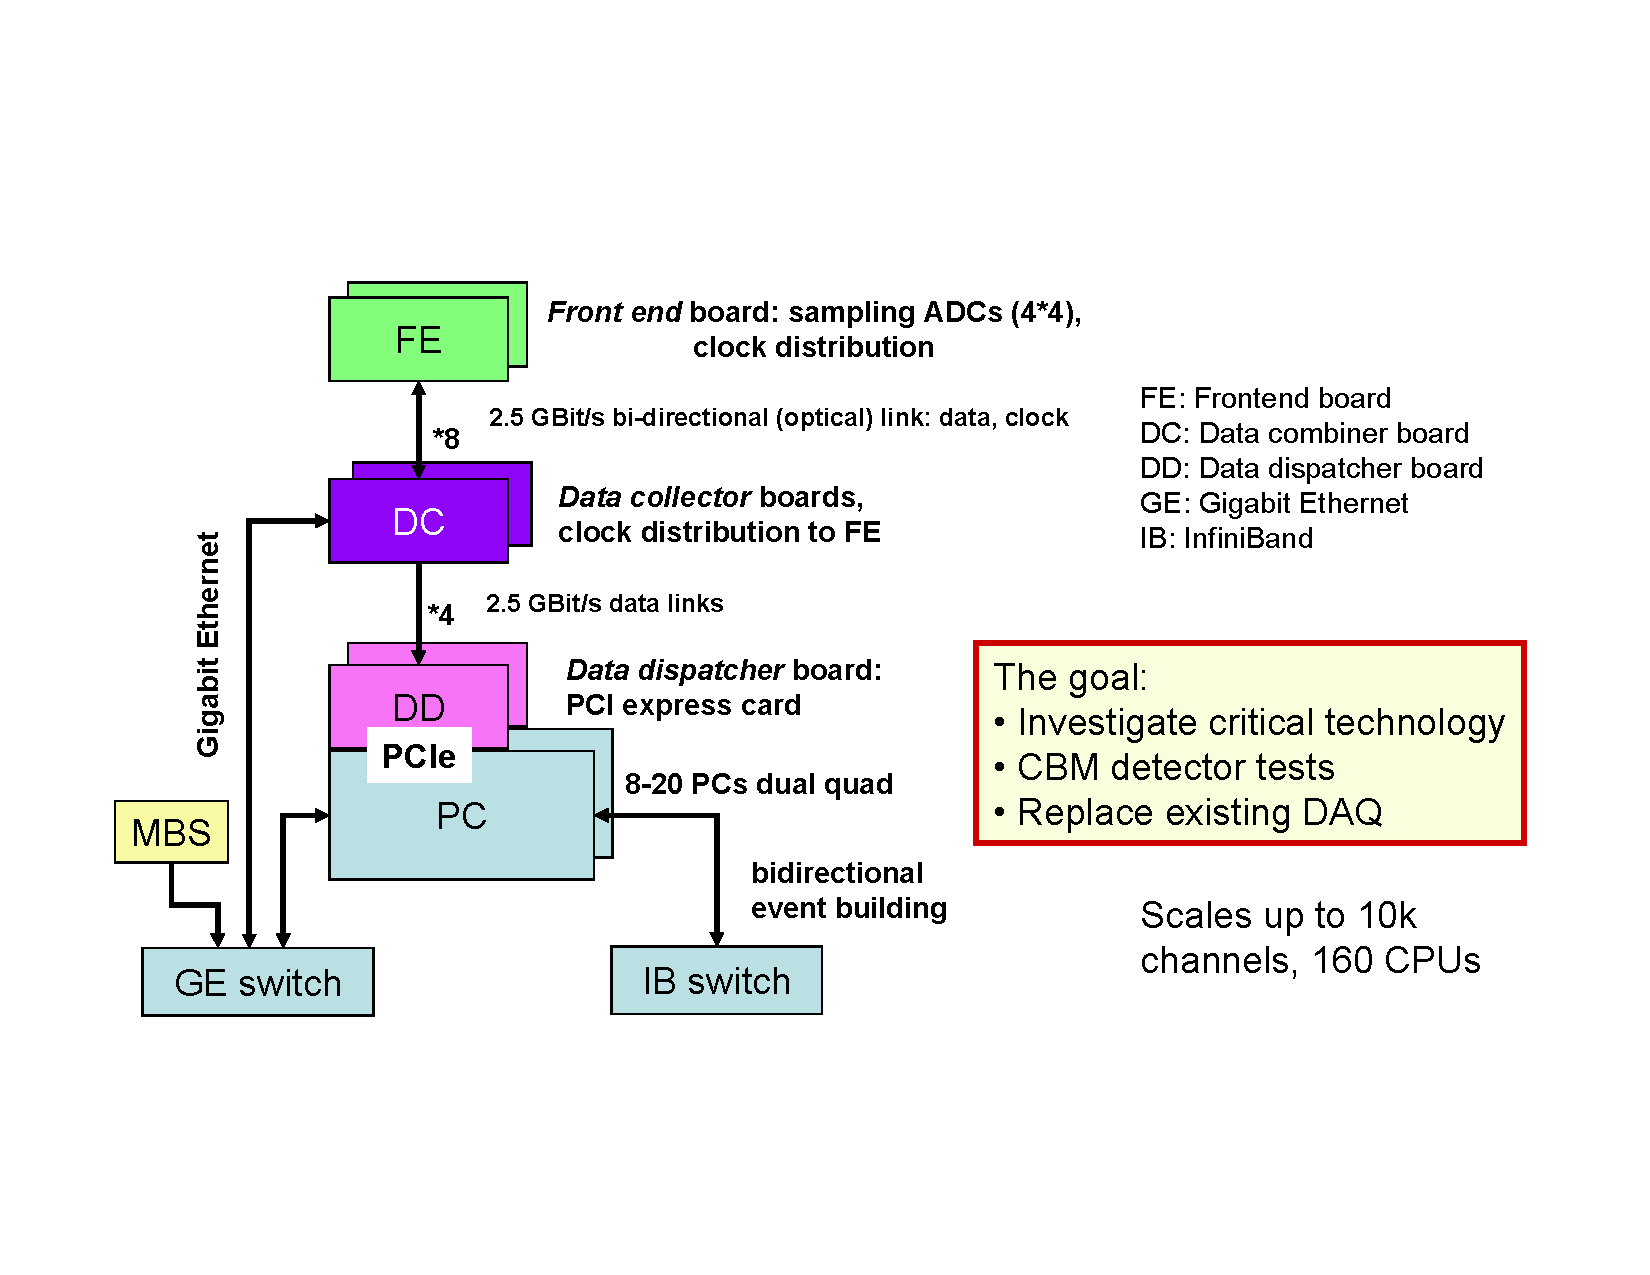
\includegraphics[width=.8\textwidth]
{dabcf-all}
\caption{\DDA~ overall data processing architecture}
\label{fig:daq-over}
\end{figure}

The system can be described in several dimensions:
\begin{compactdesc}
\item[Hardware] There are mainly three boards with different tasks but similar architecture.
\item[Data formats] The data and time stamp formats must be defined early because they are
interpreted at many occasions. A change would have big impact.
\item[Data flow models] Mechanisms how the data is moving throughout the system.
\item[Software framework] What frameworks are used. We should not start from scratch.
\item[High level software] Runs wherever Linux is running.
\item[Board level software] Mainly the FPGA codes
\item[Controls] Several sorts of controls
\end{compactdesc}

\subsection{Hardware}
The hardware components as shown in Fig.~\ref{fig:daq-over} are
summarized with their key features.
\subsubsection{Front End Electronics board FEE}
General purpose chamber-mountable board with ADCs (4*4 channels,
65 MHz sampling, 10-12 bit), FPGA (Virtex-4, PPC, Ethernet MAC,
MGT plus SDRAM, CPLD, NVRAM), plugable to preamp/chapers. A
version utilizing pipeline TDCs (ns resolution) possible. Two
clock domains: receive clock of 312.5 MHz (timing and trigger) and
sampling clock with 62.5 MHz (measurement). Four pair of LVDS
bi-directional links (625 Mbps).
\subsubsection{Data Combiner board DCB}
Four bi-directional LVDS links to FEB, Ethernet, MGT with SFP
optical link to ABB, same FPGA. A test layout of such board is shown in Fig.~\ref{fig:dcb}.
A possible connection to the between FEE and DCB boards is shown if Fig.~\ref{fig:fee-dcb}
\subsubsection{Active Buffer board ABB}
PCIe board, 4 - 8 MGT/SFP optical links to DCBs, same FPGA.
\subsubsection{Timing board}
Similar to DCB, gets optional trigger inputs, generates clock and distributes through
optical splitters to DCBs.
\subsubsection{Event builder}
Standard PC with GE, InifiniBand switch.


\subsection{Data formats}
See also \hyperref{http://www-linux.gsi.de/~mbs/main-software.pdf}{sw}{data}{Software paper}.
\subsubsection{Raw data stream}
The data must be formatted on the FEE boards to achieve the following requirements:
\begin{compactenum}
\item compressed
\item coded geographical address
\item incremental time stamps
\item time epoch markers
\end{compactenum}
The event building is done through a switched network.
Logical entities to be switched are epochs.
Data before switching may be stored/retrieved in a binary format for testing and/or
development..
It should be foreseen that data has to be reformatted before the switching, because different
subsystems might produce different data formats. Eventually the time sorting might be done.
After the switching, the event definition has to be done.
At that point all data must be repacked.
\subsubsection{Event definition data}
This intermediate format is a full time ordered compressed data stream of an epoch.
Optionally it may contain multiplicity histograms to accelerate later event definition.
Data may be stored/retrieved in this format.
\subsubsection{Event format}
After event definition events must be formatted and stored.

\subsection{Software}
\subsubsection{Board level software}
Software running on the FPGAs. The data flow from the FEE through
the DCB to the ABB is controlled by FPGAs.
\subsubsection{Data mover}
The data dispatchers (task on standard PCs with Linux) read the
data stream via PCIe from the ABB boards and send it via a fast
network (GE or IB) switch to the event builder tasks (same PCs)
using the links bi-directional.
\subsubsection{Data processing}
From the event builder task the formatted events are handed over
to data processing tasks for event filtering and archiving. These
tasks can run optionally on separate machines.
\subsection{Controls}
For the three main fields of detector controls, DAQ controls, and board controls
there are currently three products under test:
\begin{compactdesc}
\item[EPICS] Well known control system, widely used in accelarator and classical controls.
SNMP interface is available for monitoring clusters and net devices.
\item[LabView] Standard slow control at GSI.
\item[SysMES] Configuration control system developed at KIP. Has CA interface to work with
EPICS and SNMP.
\item[xDAQ] DAQ framework of CMS
\end{compactdesc}
Because it might be not possible to make a decision for one of these to be used exclusively
one should investigate/implement interoperability.
Communication standards in question:
\begin{compactitem}
\item DIM: DIM server in an EPICS IOC as first test bridge
\item CA: LabView CA client available
\item SOAP: provided by xDAQ, Java interface available.
\item CA: EPICS IOC (xDAQ application) gateway to xDAQ infospace
\end{compactitem}
The DAQ controls must provide the following functionality:
\begin{compactitem}
\item Control tasks on remote machines
\item Communicate with all tasks
\item Mechanism to store/retrieve the whole setup
\item Monitor setup, status, data flow, and performance
\item Control data flows
\item Visualization and GUI
\end{compactitem}
